\section{Gradiente desvaneciente (o que explota)}

El gradiente desvameciente o que explota en ingles \emph{Gradient descent} es un método general de minimización para cualquier función $f$. En redes neuronales el gradiente es un cálculo que nos permite saber cómo ajustar los parámetros de la red de tal forma que se minimice su desviación a la salida.
Entonces retomando lo que hacemos en el entrenamiento una vez calcuadas las salidas de las neuronas es calcular los deltas asociados a las diferentes neuronas de la red, para lo que recorremos la red hacia atrás(desde la capa de salida hasta la capa de entrada):

Con las ecuaciones que ya vimos anteriormente (insertar ecuaciones).

Una vez realizada la propagación hacia atrás de los errores, actualizamos los pesos de la red utilizando la expresión asociada al gradiente.

(insertar ecuaciones :P).

En el ajuste de un peso asociado a la entrada $x_i$ de una neurona, intervienen tres factores: 
\begin{itemize}
 \item el valor de la entrada $x_i$
 \item la derivada de su función de activación dada su entrada neta
 \item una señal de error que depende de la capa en la que nos encontremos y que proviene de las
siguientes capas de la red.
\end{itemize}

En el algoritmo de propagación de errores, partimos de una señal de error observada en la capa de salida de la red y vamos propagando esa señal de error hacia atrás por toda la red. Pudimos notar que el gradiente del error de una neurona oculta se podía calcular combinando los gradientes del error para las neuronas de la siguiente capa de la red.

Si el nivel de activación de una neurona es bajo,los pesos asociados a las sinapsis que reciben como entrada la salida
de la neurona se ajustarán lentamente.La presencia de pesos elevados en los caminos desde la neurona oculta
hasta la salida indicarán una contribución elevada al gradiente del error. En el momento en el que una neurona (sigmoidal) se satura, los gradientes del error serán muy bajos y la neurona oculta dejará de aprender, ya que los ajustes que realizamos sobre sus pesos son proporcionales a la derivada de su función de activación. En el mejor de los casos, aprenderá muy lentamente.

\begin{figure}[H]
 \centering
 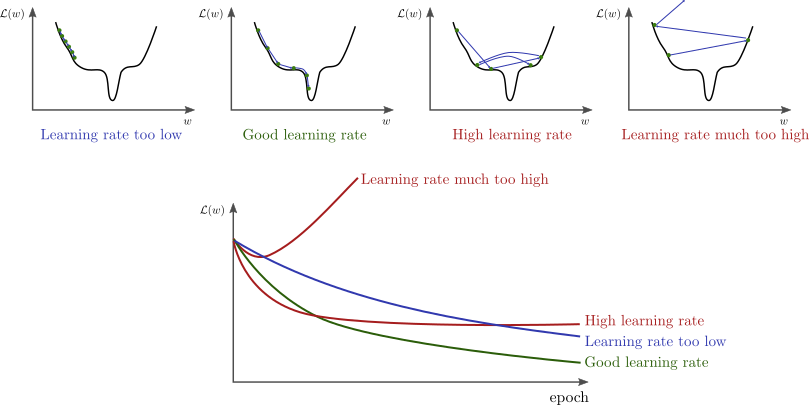
\includegraphics[scale=0.5]{../Figuras/gradiente.png}
 \caption{Rehacerla bien. por copyright..}
 \label{fig:gradiente}
\end{figure}

Lo más habitual es que las capas más alejadas de la salida de la red aprendan más lentamente que las capas más cercanas a la salida. Dado que los niveles de activación de las neuronas están acotados y los resultantados a menudo son menores que 1. En casos extremos, el gradiente será prácticamente nulo, por lo que la red será incapaz de aprender. Dandonos el 
 problema conocido como gradiente desvaneciente en inglés \emph{vanishing gradient}.

 También puede darse el caso opuesto. Si los pesos de la red aumentan en exceso durante el entrenamiento de la red (p.ej. si utilizamos una tasa de aprendizaje demasiado elevada que hace que el gradiente descendente sea inestable y diverja), los factores involucrados en el cálculo del gradiente tomarán valores mucho mayores que 1. En este caso, el problema es el contrario al gradiente devanescente y tendríamos la explosión del gradiente \emph{exploding gradient}.

 \begin{center}
 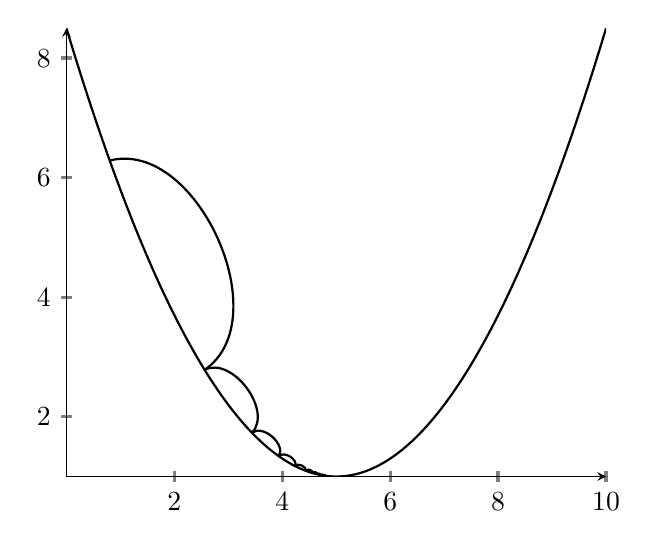
\begin{tikzpicture}
\begin{axis}[
axis lines=middle,
tick style={very thick},
]
%
%line of best fit
\addplot[thick,samples=151,domain=0:10] {0.3*(x-5)^(2) + 1}
foreach \x in {1,...,12} {coordinate[pos={0.5-1.5/pow(1+\x,2)}] (p\x)
\ifnum\x>1
(p\the\numexpr\x-1) edge[bend left=80] (p\x)
\fi};
\end{axis}
\newline
%\caption{Buena taza de aprendizaje. Desenso por el gradiente deseado.}
\end{tikzpicture}
\end{center}

\begin{figure}[H]
 \centering
 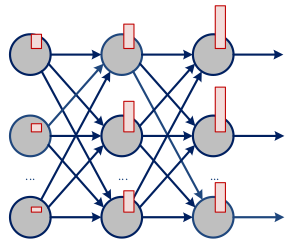
\includegraphics[scale=0.5]{../Figuras/vanish.png}
 \caption{La magnitud del gradiente varía de una capa a otra durante el entrenamiento de una red neuronal multicapa}
 \label{fig:vanish}
\end{figure}

En resumen, el aprendizaje basado en gradiente descendente usando retroporpagación puede no funcionar demasiado bien cuando el nivel de activación de una neurona j es bajo (lo que afecta al ajuste de los pesos de las neuronas que reciben como entrada la salida de la neurona j), las neuronas sigmoidales se estancan (por lo que las derivadas de sus funciones
de activación serán bajas, lo cual afecta al entrenamiento de sus pesos y, potencialmente, al de las neuronas que las preceden en la red) o la profundidad de nuestra red hace que se vea afectada por problemas como desvanecimiento o exploción del gradiente.

